% Left: two staircases 1+2+...+6 make a 6 x 7 rectangle. Right: the odd numbers as gnomons of a square;
% the gnomons grouped 1 | 3,5 | 7,9,11 | ... have areas 1, 8, 27, ...: Nicomachus's observation. Generated by figs_t0c01.py.
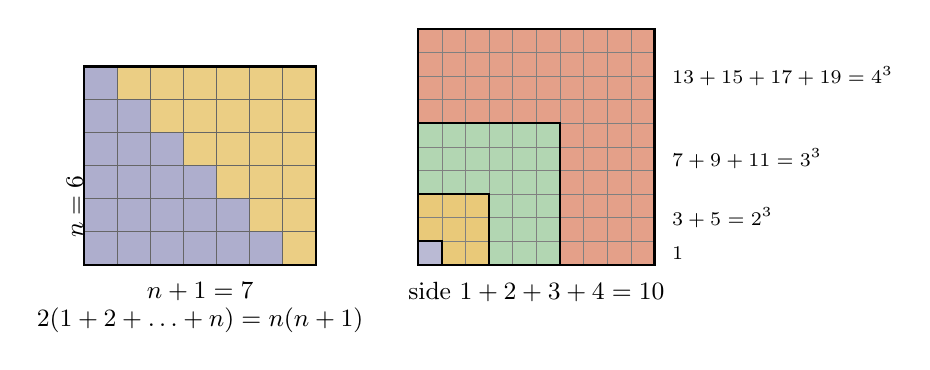
\begin{tikzpicture}
\begin{scope}
\fill[MidnightBlue!35] (0.000,-0.420) rectangle (0.420,0.000);
\fill[Goldenrod!55] (0.420,-0.420) rectangle (0.840,0.000);
\fill[Goldenrod!55] (0.840,-0.420) rectangle (1.260,0.000);
\fill[Goldenrod!55] (1.260,-0.420) rectangle (1.680,0.000);
\fill[Goldenrod!55] (1.680,-0.420) rectangle (2.100,0.000);
\fill[Goldenrod!55] (2.100,-0.420) rectangle (2.520,0.000);
\fill[Goldenrod!55] (2.520,-0.420) rectangle (2.940,0.000);
\fill[MidnightBlue!35] (0.000,-0.840) rectangle (0.420,-0.420);
\fill[MidnightBlue!35] (0.420,-0.840) rectangle (0.840,-0.420);
\fill[Goldenrod!55] (0.840,-0.840) rectangle (1.260,-0.420);
\fill[Goldenrod!55] (1.260,-0.840) rectangle (1.680,-0.420);
\fill[Goldenrod!55] (1.680,-0.840) rectangle (2.100,-0.420);
\fill[Goldenrod!55] (2.100,-0.840) rectangle (2.520,-0.420);
\fill[Goldenrod!55] (2.520,-0.840) rectangle (2.940,-0.420);
\fill[MidnightBlue!35] (0.000,-1.260) rectangle (0.420,-0.840);
\fill[MidnightBlue!35] (0.420,-1.260) rectangle (0.840,-0.840);
\fill[MidnightBlue!35] (0.840,-1.260) rectangle (1.260,-0.840);
\fill[Goldenrod!55] (1.260,-1.260) rectangle (1.680,-0.840);
\fill[Goldenrod!55] (1.680,-1.260) rectangle (2.100,-0.840);
\fill[Goldenrod!55] (2.100,-1.260) rectangle (2.520,-0.840);
\fill[Goldenrod!55] (2.520,-1.260) rectangle (2.940,-0.840);
\fill[MidnightBlue!35] (0.000,-1.680) rectangle (0.420,-1.260);
\fill[MidnightBlue!35] (0.420,-1.680) rectangle (0.840,-1.260);
\fill[MidnightBlue!35] (0.840,-1.680) rectangle (1.260,-1.260);
\fill[MidnightBlue!35] (1.260,-1.680) rectangle (1.680,-1.260);
\fill[Goldenrod!55] (1.680,-1.680) rectangle (2.100,-1.260);
\fill[Goldenrod!55] (2.100,-1.680) rectangle (2.520,-1.260);
\fill[Goldenrod!55] (2.520,-1.680) rectangle (2.940,-1.260);
\fill[MidnightBlue!35] (0.000,-2.100) rectangle (0.420,-1.680);
\fill[MidnightBlue!35] (0.420,-2.100) rectangle (0.840,-1.680);
\fill[MidnightBlue!35] (0.840,-2.100) rectangle (1.260,-1.680);
\fill[MidnightBlue!35] (1.260,-2.100) rectangle (1.680,-1.680);
\fill[MidnightBlue!35] (1.680,-2.100) rectangle (2.100,-1.680);
\fill[Goldenrod!55] (2.100,-2.100) rectangle (2.520,-1.680);
\fill[Goldenrod!55] (2.520,-2.100) rectangle (2.940,-1.680);
\fill[MidnightBlue!35] (0.000,-2.520) rectangle (0.420,-2.100);
\fill[MidnightBlue!35] (0.420,-2.520) rectangle (0.840,-2.100);
\fill[MidnightBlue!35] (0.840,-2.520) rectangle (1.260,-2.100);
\fill[MidnightBlue!35] (1.260,-2.520) rectangle (1.680,-2.100);
\fill[MidnightBlue!35] (1.680,-2.520) rectangle (2.100,-2.100);
\fill[MidnightBlue!35] (2.100,-2.520) rectangle (2.520,-2.100);
\fill[Goldenrod!55] (2.520,-2.520) rectangle (2.940,-2.100);
\draw[step=0.42cm,black!60,thin] (0,-2.520) grid (2.940,0);
\draw[thick] (0,-2.520) rectangle (2.940,0);
\node[font=\small,anchor=north] at (1.470,-2.620) {$n+1=7$};
\node[font=\small,anchor=east,rotate=90] at (-0.12,-1.260) {$n=6$};
\node[font=\small] at (1.470,-3.220) {$2(1+2+\dots+n)=n(n+1)$};
\end{scope}
\begin{scope}[xshift=4.240cm,yshift=-2.520cm]
\fill[MidnightBlue!30] (0.000,0.000) rectangle (0.300,0.300);
\fill[Goldenrod!60] (0.000,0.300) rectangle (0.300,0.600);
\fill[Goldenrod!60] (0.300,0.300) rectangle (0.600,0.600);
\fill[Goldenrod!60] (0.300,0.000) rectangle (0.600,0.300);
\fill[Goldenrod!60] (0.000,0.600) rectangle (0.300,0.900);
\fill[Goldenrod!60] (0.300,0.600) rectangle (0.600,0.900);
\fill[Goldenrod!60] (0.600,0.600) rectangle (0.900,0.900);
\fill[Goldenrod!60] (0.600,0.000) rectangle (0.900,0.300);
\fill[Goldenrod!60] (0.600,0.300) rectangle (0.900,0.600);
\fill[ForestGreen!35] (0.000,0.900) rectangle (0.300,1.200);
\fill[ForestGreen!35] (0.300,0.900) rectangle (0.600,1.200);
\fill[ForestGreen!35] (0.600,0.900) rectangle (0.900,1.200);
\fill[ForestGreen!35] (0.900,0.900) rectangle (1.200,1.200);
\fill[ForestGreen!35] (0.900,0.000) rectangle (1.200,0.300);
\fill[ForestGreen!35] (0.900,0.300) rectangle (1.200,0.600);
\fill[ForestGreen!35] (0.900,0.600) rectangle (1.200,0.900);
\fill[ForestGreen!35] (0.000,1.200) rectangle (0.300,1.500);
\fill[ForestGreen!35] (0.300,1.200) rectangle (0.600,1.500);
\fill[ForestGreen!35] (0.600,1.200) rectangle (0.900,1.500);
\fill[ForestGreen!35] (0.900,1.200) rectangle (1.200,1.500);
\fill[ForestGreen!35] (1.200,1.200) rectangle (1.500,1.500);
\fill[ForestGreen!35] (1.200,0.000) rectangle (1.500,0.300);
\fill[ForestGreen!35] (1.200,0.300) rectangle (1.500,0.600);
\fill[ForestGreen!35] (1.200,0.600) rectangle (1.500,0.900);
\fill[ForestGreen!35] (1.200,0.900) rectangle (1.500,1.200);
\fill[ForestGreen!35] (0.000,1.500) rectangle (0.300,1.800);
\fill[ForestGreen!35] (0.300,1.500) rectangle (0.600,1.800);
\fill[ForestGreen!35] (0.600,1.500) rectangle (0.900,1.800);
\fill[ForestGreen!35] (0.900,1.500) rectangle (1.200,1.800);
\fill[ForestGreen!35] (1.200,1.500) rectangle (1.500,1.800);
\fill[ForestGreen!35] (1.500,1.500) rectangle (1.800,1.800);
\fill[ForestGreen!35] (1.500,0.000) rectangle (1.800,0.300);
\fill[ForestGreen!35] (1.500,0.300) rectangle (1.800,0.600);
\fill[ForestGreen!35] (1.500,0.600) rectangle (1.800,0.900);
\fill[ForestGreen!35] (1.500,0.900) rectangle (1.800,1.200);
\fill[ForestGreen!35] (1.500,1.200) rectangle (1.800,1.500);
\fill[BrickRed!35] (0.000,1.800) rectangle (0.300,2.100);
\fill[BrickRed!35] (0.300,1.800) rectangle (0.600,2.100);
\fill[BrickRed!35] (0.600,1.800) rectangle (0.900,2.100);
\fill[BrickRed!35] (0.900,1.800) rectangle (1.200,2.100);
\fill[BrickRed!35] (1.200,1.800) rectangle (1.500,2.100);
\fill[BrickRed!35] (1.500,1.800) rectangle (1.800,2.100);
\fill[BrickRed!35] (1.800,1.800) rectangle (2.100,2.100);
\fill[BrickRed!35] (1.800,0.000) rectangle (2.100,0.300);
\fill[BrickRed!35] (1.800,0.300) rectangle (2.100,0.600);
\fill[BrickRed!35] (1.800,0.600) rectangle (2.100,0.900);
\fill[BrickRed!35] (1.800,0.900) rectangle (2.100,1.200);
\fill[BrickRed!35] (1.800,1.200) rectangle (2.100,1.500);
\fill[BrickRed!35] (1.800,1.500) rectangle (2.100,1.800);
\fill[BrickRed!35] (0.000,2.100) rectangle (0.300,2.400);
\fill[BrickRed!35] (0.300,2.100) rectangle (0.600,2.400);
\fill[BrickRed!35] (0.600,2.100) rectangle (0.900,2.400);
\fill[BrickRed!35] (0.900,2.100) rectangle (1.200,2.400);
\fill[BrickRed!35] (1.200,2.100) rectangle (1.500,2.400);
\fill[BrickRed!35] (1.500,2.100) rectangle (1.800,2.400);
\fill[BrickRed!35] (1.800,2.100) rectangle (2.100,2.400);
\fill[BrickRed!35] (2.100,2.100) rectangle (2.400,2.400);
\fill[BrickRed!35] (2.100,0.000) rectangle (2.400,0.300);
\fill[BrickRed!35] (2.100,0.300) rectangle (2.400,0.600);
\fill[BrickRed!35] (2.100,0.600) rectangle (2.400,0.900);
\fill[BrickRed!35] (2.100,0.900) rectangle (2.400,1.200);
\fill[BrickRed!35] (2.100,1.200) rectangle (2.400,1.500);
\fill[BrickRed!35] (2.100,1.500) rectangle (2.400,1.800);
\fill[BrickRed!35] (2.100,1.800) rectangle (2.400,2.100);
\fill[BrickRed!35] (0.000,2.400) rectangle (0.300,2.700);
\fill[BrickRed!35] (0.300,2.400) rectangle (0.600,2.700);
\fill[BrickRed!35] (0.600,2.400) rectangle (0.900,2.700);
\fill[BrickRed!35] (0.900,2.400) rectangle (1.200,2.700);
\fill[BrickRed!35] (1.200,2.400) rectangle (1.500,2.700);
\fill[BrickRed!35] (1.500,2.400) rectangle (1.800,2.700);
\fill[BrickRed!35] (1.800,2.400) rectangle (2.100,2.700);
\fill[BrickRed!35] (2.100,2.400) rectangle (2.400,2.700);
\fill[BrickRed!35] (2.400,2.400) rectangle (2.700,2.700);
\fill[BrickRed!35] (2.400,0.000) rectangle (2.700,0.300);
\fill[BrickRed!35] (2.400,0.300) rectangle (2.700,0.600);
\fill[BrickRed!35] (2.400,0.600) rectangle (2.700,0.900);
\fill[BrickRed!35] (2.400,0.900) rectangle (2.700,1.200);
\fill[BrickRed!35] (2.400,1.200) rectangle (2.700,1.500);
\fill[BrickRed!35] (2.400,1.500) rectangle (2.700,1.800);
\fill[BrickRed!35] (2.400,1.800) rectangle (2.700,2.100);
\fill[BrickRed!35] (2.400,2.100) rectangle (2.700,2.400);
\fill[BrickRed!35] (0.000,2.700) rectangle (0.300,3.000);
\fill[BrickRed!35] (0.300,2.700) rectangle (0.600,3.000);
\fill[BrickRed!35] (0.600,2.700) rectangle (0.900,3.000);
\fill[BrickRed!35] (0.900,2.700) rectangle (1.200,3.000);
\fill[BrickRed!35] (1.200,2.700) rectangle (1.500,3.000);
\fill[BrickRed!35] (1.500,2.700) rectangle (1.800,3.000);
\fill[BrickRed!35] (1.800,2.700) rectangle (2.100,3.000);
\fill[BrickRed!35] (2.100,2.700) rectangle (2.400,3.000);
\fill[BrickRed!35] (2.400,2.700) rectangle (2.700,3.000);
\fill[BrickRed!35] (2.700,2.700) rectangle (3.000,3.000);
\fill[BrickRed!35] (2.700,0.000) rectangle (3.000,0.300);
\fill[BrickRed!35] (2.700,0.300) rectangle (3.000,0.600);
\fill[BrickRed!35] (2.700,0.600) rectangle (3.000,0.900);
\fill[BrickRed!35] (2.700,0.900) rectangle (3.000,1.200);
\fill[BrickRed!35] (2.700,1.200) rectangle (3.000,1.500);
\fill[BrickRed!35] (2.700,1.500) rectangle (3.000,1.800);
\fill[BrickRed!35] (2.700,1.800) rectangle (3.000,2.100);
\fill[BrickRed!35] (2.700,2.100) rectangle (3.000,2.400);
\fill[BrickRed!35] (2.700,2.400) rectangle (3.000,2.700);
\draw[step=0.3cm,black!50,very thin] (0,0) grid (3.000,3.000);
\draw[thick] (0,0) rectangle (0.300,0.300);
\draw[thick] (0,0) rectangle (0.900,0.900);
\draw[thick] (0,0) rectangle (1.800,1.800);
\draw[thick] (0,0) rectangle (3.000,3.000);
\node[font=\scriptsize,anchor=west] at (3.100,0.150) {$1$};
\node[font=\scriptsize,anchor=west] at (3.100,0.600) {$3+5=2^3$};
\node[font=\scriptsize,anchor=west] at (3.100,1.350) {$7+9+11=3^3$};
\node[font=\scriptsize,anchor=west] at (3.100,2.400) {$13+15+17+19=4^3$};
\node[font=\small,anchor=north] at (1.500,-0.1) {side $1+2+3+4=10$};
\end{scope}
\end{tikzpicture}
